\section{Méthodes numériques}
\subsection{Introduction}
Dans le contexte des projets industriels, la réalisation de campagnes de tests pour dimensionner les systèmes engendre des coûts très importants. Par conséquents des modèles physiques sont de plus en plus utilisés durant les phases de conception des produits dans l'optique de limiter le plus possible les tests en laboratoire et de circonscrire dans la mesure du possible leur utilisation aux seules phases de certifications.\\

Les phénomènes physiques étudiés sont modélisés mathématiquement au moyen d'Equations au Dérivées Partielles (EDP), qui ont pour objet de lier les variations spatiales et temporelles des quantités observées.

A titre d'exemple, les équations de Navier-Stokes conservatives, qui modélisent un écoulement fluide, peuvent s'écrire de la manière suivante:

\begin{equation}
    \frac{\partial W}{\partial t} + \nabla . F(W) -\nabla\left( G(W,\nabla W)\right)=0
    \label{eq:NS}
\end{equation}

où $W$ représente le vecteur d'état (vitesse d'écoulement, énergie...), $F$ donne le flux de ce vecteur d'état et $G$ est un terme de viscosité.\\

En règle général on ne dispose pas de solution analytique des EDP pour des conditions initiales et des conditions de bords quelconques. C'est pour cela que l'on introduit les simulations numériques qui permettent de calculer des solutions approchées de ses équations.\\

Le projet sur lequel nous sommes intervenus se focalise sur le développement d'un code dit de \emph{Computational Fluid Dynamics} (CFD) qui s'intéresse spécifiquement à ces problèmes de modélisation d'écoulement fluide.\\

Lorsqu'on ne prend pas en compte le terme visqueux dans l'équation (\ref{eq:NS}) et qu'on se place en dimension 1D, cette équation se ré-écrit sous la forme d'une équation d'advection:

\begin{equation} 
    \frac{\partial W}{\partial t}+\frac{\partial \mathrm{F}(W)}{\partial x}=0
    \label{eq:advct}
\end{equation}

Cette équation simplifiée du modèle précédent nous a servi de cas test basique tout au long de notre étude car elle présente l'avantage d'être à la fois proche des problématiques de dynamique des fluides de nos clients ainsi que de posséder des solutions analytique ce qui nous a permis d'évaluer la pertinence de nos méthodes numériques.
%idée général des coût de test phy élevés donc simu
%modélisation de la physique par les EDP
%approche numérique si trop complexe pour avoir une sol analytique
\subsubsection{Couplage spatio-temporel}
Il est possible d'isoler dans les équations que nous étudions ici une partie traitant de l'évolution temporelle et une partie se focalisant sur les variations spatiales. Il est notamment possible de reformuler l'équation (\ref{eq:advct}) de la manière suivante:

\begin{equation}
\frac{\partial W}{\partial t} = -\frac{\partial F(W)}{\partial x}
\label{eq:SpTmp}
\end{equation}

la partie temporelle étant contenue dans le membre de gauche et la partie spatiale dans le membre de droite.

En règle générale, les démarches numériques exposées dans la littérature se focalisent en premier lieu sur l'un ou l'autre de ces aspects.

En ce qui concerne le code développé dans le cadre du projet JAGUAR de notre client c'est l'aspect spatial qui a été particulièrement étudié au travers des méthodes de \emph{Spectral Difference}, exposées dans la sous-section suivante. L'objet d'un PIE précédent consistait précisément à implémenter une méthode de discrétisation de l'opérateur différentiel spatial du membre de gauche de l'équation (\ref{eq:SpTmp}).

Une fois cette étape de discrétisation spatiale réalisée, on peut se ramener à l'étude d'une Equation Différentielle Ordinaire (EDO) de la forme:

\begin{equation}
\left\{
    \begin{aligned}
    \dot{u} = f(t,u)&\\
    u(0) = u_0, &\quad u_0\in \mathbb{R}^n
    \end{aligned}
    \right.
    \label{eq:EDO}
\end{equation}

%Comme expliqué précédemment, notre objectif était de trouver une méthode temporelle en adéquation avec la précision des méthodes spatiales développées par le client. Vérifié la validité du couplage spatio-temporel des différentes méthodes considérées ici faisait donc partie des enjeux cruciaux pour satisfaire notre client.\\
C'est la possibilité d'étudier en parallèle à la fois de nouvelles méthodes numériques temporelles ainsi qu'un traitement du couplage spatio-temporel qui a motivé notre choix de nous répartir en deux équipes distincts.

Dans la suite du rapport sont donc exposés en premier lieu les méthodes de différences spectrales, puis rappels sur les méthodes numériques d'intégration des EDO classiques suivi par l'étude des méthode d'intégrations exponentielles plus récentes et enfin les résultats que nous avons obtenu après implémentation.
%description des eq du problème,
%séparation spatio-temp, en général étudié spéparement
%réduction au EDO
\subsubsection{Notions essentielles d'analyse numérique}
Comme mentionné précédemment, l'utilisation de schémas numériques est souvent indispensable aussi bien pour la résolution d'EDP que pour la résolution d'EDO. Avant de passer au parties suivantes, nous rappelons ici quelques notions essentielles d'analyse numérique.\\

On se place ici dans le cas très simple où l'on considère le problème suivant:
\begin{equation}
\left\{
    \begin{aligned}
        \dot{u} = A u, \quad  A \in \mathcal{M}_n(\mathbb{R})\\
        u(0) = u_0, \quad u_0 \in \mathbb{R}^n
    \end{aligned}
\right.
\label{eq:lin}
\end{equation}

Cette équation différentielle ordinaire à pour solution la fonction
$$
u(t) = e^{A t}u_0, \quad t\in \mathbb{R}
$$
et est stable ssi son spectre est inclus dans le demi-plan gauche de l'espace complexe $\mathbb{C}$ (i.e. $\forall \lambda \in \sigma(A), Re (\lambda) \leq 0$). Si les valeurs du spectre sont strictement contenues dans $\mathbb{C}^- = \{z\in \mathbb{C}, Re(z)<0\}$, alors la solution du problème est asymptotiquement stable et converge exponentiellement vite vers $0$.\\

Une façon intuitive de discrétiser le problème selon un pas de temps $\Delta t$ est la suivante:
\begin{equation}
    \frac{u_{n+1}-u_n}{\Delta t} = A u_n 
    \label{eq:Euler}
\end{equation}
Il s'agit du schéma d'Euler.

En posant pour $n\in \mathbb{N}$ $t_n = n \Delta t$, on peut montrer par un développement limité qu'une solution du problème (\ref{eq:lin}) vérifie:
$$
\frac{u(t_{n+1}) -u(t_n)}{\Delta t} = \frac{1}{\Delta t}\left(u(t_n) + \Delta t \dot{u}(t_n) +o(\Delta t) - u(t_n)\right) = Au_n +o(1)
$$
Autrement dit une solution de (\ref{eq:lin}) vérifie le schéma (\ref{eq:Euler}) à un terme résiduel prés qui converge vers 0 lorsque $\Delta t \rightarrow 0$. Réciproquement, on peut montrer qu'une fonction vérifie l'équation (\ref{eq:Euler}) seulement si elle vérifie à un terme résiduel près le système (\ref{eq:lin}). Cela caractérise la notion de \emph{consistance} qui représente intuitivement la capacité du schéma numérique à bien restituer le comportement local des solutions que l'on cherche à simuler lorsque l'on fait tendre le pas de temps $\Delta t$ vers.\\

Cette erreur locale sera inévitablement reproduite à chaque itération de notre schéma numérique et s'accumulera progressivement. On peut cependant attendre du schéma qu'il n'amplifie pas déraisonnablement cet écart. C'est ce qui correspond intuitivement à la notion de \emph{stabilité}.  
%rappel utilité
%cas très simple
%convergence: notions de stabilité et de consistance
%deux grandes approches: explicite vs implicite
\subsection{Méthodes spectrales}

\paragraph{}
Les méthodes spectrales ont été le sujet d'un précédent PIE, sur lequel nous nous basons dans le cadre de notre travail. Dans cette partie nous allons présenter certaines propriétés de la méthode des différence spectrales (méthode SD).

    \subsubsection{Intérêt}
    \paragraph{}
    Les méthodes spectrales se distinguent des autres méthodes car elles permettent de conserver des propriétés physiques des phénomènes étudiés. Notamment en mécanique des fluides une des propriétés importante est la conservation du flux. Cette méthode permet aussi un gain de temps de calcul considérable par rapport au différence finies. Et les performances d'un solveur étant en partie lié à la rapidité de résolution on comprend l'intérêt porté à ces méthodes.
    \paragraph{}
    En terme de précision nous pouvons obtenir des ordres très élevés avec ces méthodes. Car on cherche la solution sous forme d'une combinaison linéaire sur des fonctions de base et que ces fonctions sont définies par cellules. 

    \subsubsection{Formalisme et Définition}
    \paragraph{}
    Comme nous l'avons vu les méthodes spectrales permettent d'assurer la continuité du flux aux interfaces. Elles sont donc particulièrement intéressantes dans les cas des EDP de type conservatives, rencontrés dans les problèmes de nos clients. Par exemple on peut considérer l'équation aux dérivées partielles suivante en 1D :
    $$\frac{\partial W}{\partial t} + \frac{\partial \mathrm{F}\left(W\right)}{\partial x} = 0$$
    On retrouve l'équation \ref{eq:advct}, où $W$ est la grandeur considérée et F le flux qui dépend de $W$.
    \paragraph{}
    Les méthodes spectrales supposent quand dans chaque cellule du domaine de calcul il y ait p + 1 degrés de liberté pour définir la solution ainsi que q + 1 degrés de liberté pour définir le flux. A un instant donné, les grandeurs F et $W$ sont approximées par des fonctions polynomiales $\mathrm{F}_N$ et $W_N$ dans la cellule $N$. Ce sont alors des polynômes de degrés respectifs p et q :
    \begin{equation}
    \begin{split}
        W_N\left(x, t\right) &= \sum_{i = 0}^p w_i\left(t\right)x^i \\
            \mathrm{F}_N\left(x, t\right) &= \sum_{i = 0}^q a_i\left(t\right)x^i
    \end{split}
    \label{eq:sol_flux_as_polynomials}
    \end{equation}
    \paragraph{}
    La résolution du problème dans chaque maille ne se fait pas dans l'espace réel mais dans un espace isoparamétrique, qui est normalisé. Dans notre cas, la cellule isoparamétrique est le segment [-1, 1] et le passage d'un espace à l'autre s'effectue par une homothétie et une translation. 
    \paragraph{}
    Des propriétés importantes de ce formalisme sont établies : 
    \begin{itemize}[label=\textbullet]
           \item Consistance du schéma : l'approximation polynomiale (équation \ref{eq:sol_flux_as_polynomials}) et l'équation du problème (équation \ref{eq:advct}) impliquent une condition sur les degrés des polynômes solution et flux : q~=~p~+~1
           \item Conservation du flux : il faut que le flux se conserve aux interfaces, il vient donc : $\mathrm{F}_{N-1}(1)=\mathrm{F}_{N}(-1)$ et $\mathrm{F}_{N}(1)=\mathrm{F}_{N+1}(-1)$
    \end{itemize}
    \begin{figure}
        \centering
        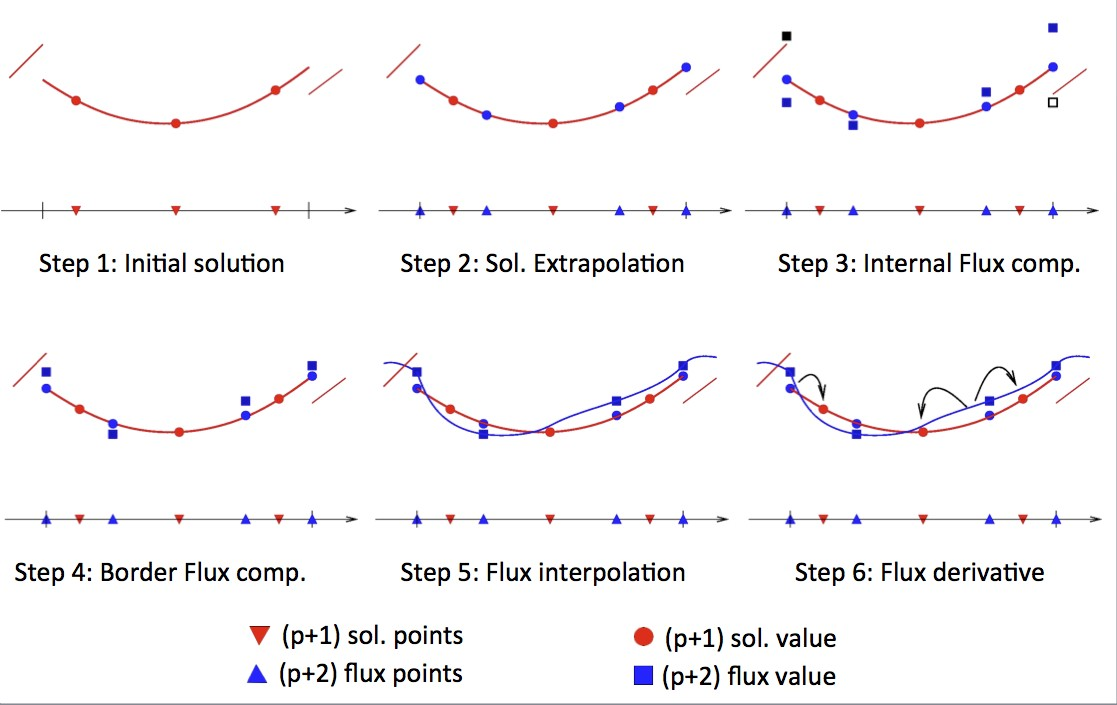
\includegraphics[width=0.8\textwidth]{images/Meth_spectrale.jpg}
          \caption{Schématisation de la méthode} 
    \label{fig:meth_spectrale}
    \end{figure}
    \paragraph{}
    Une brève description de la méthode, illustrée par la figure \ref{fig:meth_spectrale}, permettra de comprendre le fonctionnement.\\
    \textbf{Étape 1 :} Initialisation de la solution dans la cellule avec un polynôme de degré p aux p~+~1 points solution\\
    \textbf{Étape 2 :} Extrapolation de la solution aux p~+~2 points flux, intercalés entre les p~+~1 points solution et positionnés aux extrémités de la cellule, par le polynôme de degré p basé sur la solution\\
    \textbf{Étape 3 :} Calcul du flux aux p~+~2 points flux grâce aux valeurs de la solution interpolée\\
    \textbf{Étape 4 :} Résolution du problème de Riemann pour calculer les flux communs aux interfaces et assurer la continuité du flux sur le domaine\\
    \textbf{Étape 5 :} Interpolation de ce flux continu aux p~+~2 points flux pour obtenir un polynôme de degré p~+~1 le représentant\\
    \textbf{Étape 6 :} Dérivation de ce polynôme de degré p~+~1 pour obtenir un polynôme de degré p représentant la dérivée du flux, et évaluation de ce polynôme en les p~+~1 points solutions\\
    Finalement, on part d'un polynôme représentant $W$ de degré p et on obtient un polynôme représentant la dérivée du flux F lui aussi de degré p.


\subsection{Méthodes temporelles}
\subsubsection{Méthodes classiques}

Dans cette section nous allons présenter les méthodes numériques de résolution temporelles qui sont les plus utilisées à l'heure actuelle. Nous savons que la principale difficulté de ces méthodes est de concilier ordre élevé et stabilité, ce qui permettrai d'augmenter la précision des calculs de logiciel de CFD. \\ 
Pour cela nous allons d'une part étudier une méthode explicite dite de Runge-Kutta (RK) et d'autre part une méthode implicite dite Backward Differentiation Formula (BDF).
La méthode BDF est d'avantage utilisée pour la résolution de phénomènes à évolution rapide qui vont tendre lentement vers une position d'équilibre (équations raides). Tandis que la méthode de Runge-Kutta est plus utilisée pour des problèmes d'advection diffusion. 

\subsubsection{Méthode de Runge-Kutta Explicite (RK)}

Il s'agit d'une méthode d'analyse numérique élaborée par Carl Runge et Martin W. Kutta en 1901.
En tant que méthode explicite, elle détermine la solution à t +  $\Delta$t en fonction de la valeur de la fonction en t. Le problème se formalise de la manière suivante :

\begin{equation}
    y(t + \Delta t) = F(y(t))
\end{equation}

Son caractère explicite donne également qu'elle sera conditionnellement stable. Cela signifie que sous les conditions données par Lax la solution ne convergera que pour des valeurs suffisamment petites de $\Delta$t. De cette manière, le coût de calcul provient du nombre élevé d'itération à cause du petit pas de temps.

Considérons le problème suivant :

\begin{equation}
    y' = f(t, y),    y(t_0) = y_0
\end{equation}

Soit $(tn)_{n \in [0, N]}$ une discrétisation de $[t_0, t_N]$ de pas $\Delta t$. En notant $t_{n,i} = t_n + c_i . \Delta t$, on a pour solutions exactes de y :

\begin{equation}
    y(t_{n,i}) = y(t_n) + \Delta t \int_{0}^{c_i} f(t_n + uh_n, y(t_n + uh_n)) \, \mathrm{d}u
\end{equation}
et
\begin{equation}
    y(t_{n + 1}) = y(t_n) + \Delta t \int_{0}^{1} f(t_n + uh_n, y(t_n + uh_n)) \, \mathrm{d}u
\end{equation}

On peut évaluer numériquement ces équations par une méthode de quadrature en introduisant s "étages". Ainsi, la méthode de Runge-Kutta est en quelque sorte une méthode à "sous-pas" multiples. De cette manière et en posant les coefficients $a_{i, k}$ et $b_i$,  on obtient la méthode de Runge-Kutta d'ordre s:

\begin{equation}
    y_{n+1} = y_n + \Delta t \sum_{i=1}^{s} b_ik_i
\end{equation}
avec,\\
    $k_i = f(t_n + c_i\Delta t, y_n + \Delta t \sum_{k=1}^{i-1} a_{i,k}k_k)$

Les coefficients de la méthode sont donnés par le tableau de Butcher. Nous remarquerons que la méthode de Runge-Kutta à l'ordre 1 (RK1) est le schéma d'Euler explicite.

La méthode usuelle de Runge-Kutta explicite est la méthode d'ordre 4 (RK4) qui est donnée par l'équation suivante:

\begin{equation}
    y_{n+1} = y_n + \frac{\Delta t}{6}(k_1 + 2k_2 + 2k_3 + k_4)
\end{equation}
où,\\
$k_1 = f(t_n, y_n)$\\
$k_2 = f(t_n + \frac{\Delta t}{2}, y_n + \frac{\Delta t}{2}k_1)$\\
$k_3 = f(t_n + \frac{\Delta t}{2}, y_n + \frac{\Delta t}{2}k_2)$\\
$k_4 = f(t_n + \Delta t, y_n + \Delta tk_3)$

Cette méthode est d'ordre 4, ce qui signifie que l'erreur totale accumulée est de l'ordre de $\Delta t^4$.

\begin{figure}[h]
    \centering
    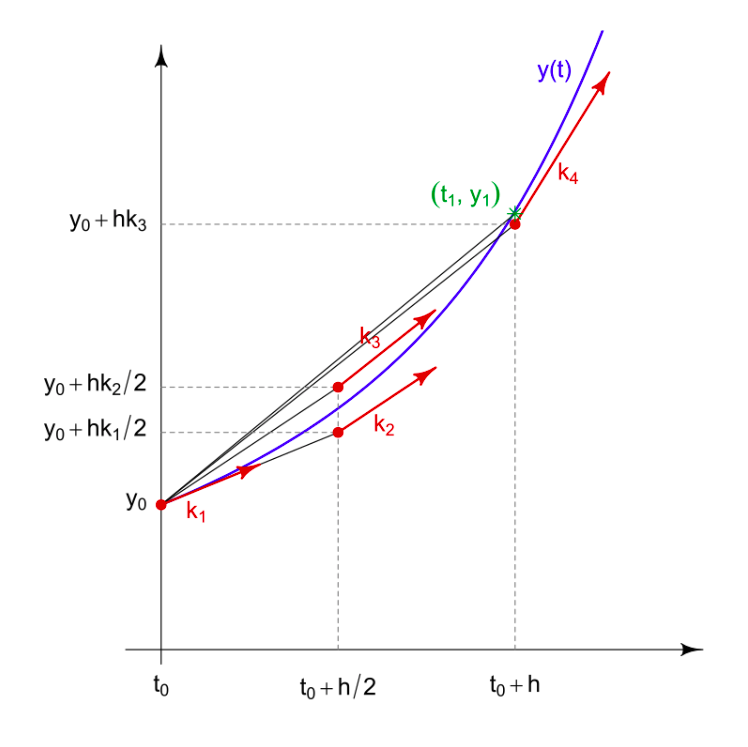
\includegraphics[width=0.5\textwidth]{images/RK_pentes.png}
    \caption{\textit{Slopes used by the classical Runge-Kutta method}, HilberTraum}
\label{fig:pentes_rk}
\end{figure}

La figure \ref{fig:pentes_rk} nous permet de réaliser que $y_{n+1}$ est calculé comme étant la somme $y_n$ et du produit entre $\Delta t$ et la pente approchée par la moyenne pondérée des pentes $k_i$. De cette manière :
\begin{itemize}
    \item $k_1$ est la pente au début de l'intervalle
    \item $k_2$ est la pente au milieu de l'intervalle en utilisant $k_1$ pour calculer $y(t_n + \frac{\Delta t}{2}$)
    \item $k_3$ est la pente au milieu de l'intervalle en utilisant $k_2$ pour calculer $y(t_n + \frac{\Delta t}{2}$)
    \item $k_4$ est la pente à la fin de l'intervalle
\end{itemize}

Le comportement des méthodes numériques sur les équations raides peut être analysé en appliquant ces méthodes à l'équation de test $y' = Ay$ sous réserve de la condition initiale y(0) = 1 avec $A \in \mathbb{C}$. La solution de cette équation est $y (t) = e^{At}$. Cette solution se rapproche de zéro lorsque t tend vers l'infini si $\mathrm{Re}(A)<0$. Si la méthode numérique présente également ce comportement, alors la méthode est dite A-stable.

\begin{figure}[h!]
    \centering
    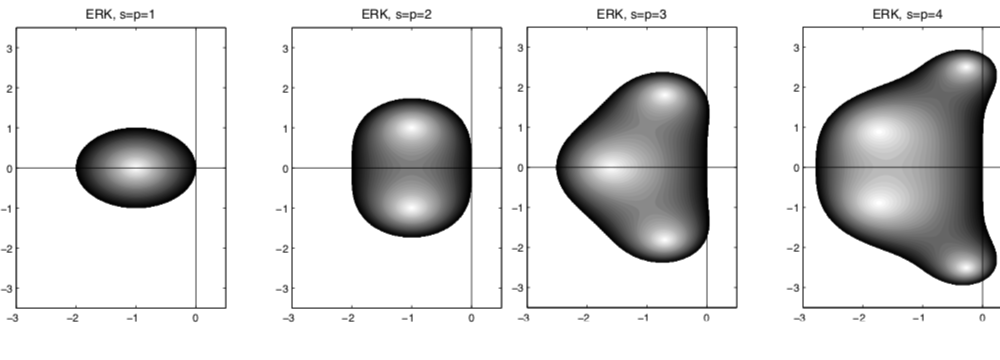
\includegraphics[width=\textwidth]{images/astab_rk.png}
    \caption{\textit{Stability of Runge-Kutta Methods}, Utrecht University}
\label{fig:astab_rk}
\end{figure}

La partie grisée de la figure \ref{fig:astab_rk} indique les valeurs de A pour lesquelles la solution numérique de y tend vers 0 respectivement sous RK1, RK2, RK3 et RK4. On remarque donc que la méthode de Runge-Kutta est conditionnellement A-Stable quelque soit son ordre. Pour cette raison, nous allons introduire une autre méthode d'analyse numérique usuelle afin d'obtenir une stabilité inconditionnelle et pouvoir traiter les cas raides.

\subsubsection{Méthode de Backward Differentiation Formula (BDF)}

Il s'agit d'une méthode d'analyse numérique élaborée par Charles F. Curtiss et Joseph O. Hirschfelder en 1952.
En tant que méthode implicite, elle détermine la solution à t +  $\Delta$t en résolvant une équation prenant en compte la valeur de la fonction en t et en t +  $\Delta$t. Le problème se formalise de la manière suivante : 

\begin{equation}
    G(y(t), y(t+\Delta t)) = 0
\end{equation}

Son caractère implicite donne également qu'elle sera inconditionnellement stable, en tout cas pour les méthodes d'ordre inférieur ou égal à 2. De cette manière, le coût de calcul provient de l'évaluation numérique de la racine de G, par une méthode de Newton par exemple.

Considérons le problème suivant :

\begin{equation}
    y' = f(t, y),    y(t_0) = y_0
\end{equation}

La méthode BDF est quand à elle une méthode à pas multiples. En posant les coefficients $a_k$ et $\beta$,  on obtient la méthode de BDF d'ordre s:

\begin{equation}
    \sum_{i=1}^{s} a_k y_{n+k} = \Delta t \beta f(t_{n+s}, y_{n+s})
\end{equation}

Les coefficients de la méthode sont donnés par le polynôme d'interpolation de Langrange. Nous remarquerons que la méthode BDF à l'ordre 1 (BDF1) est le schéma d'Euler implicite.

La méthode usuelle BDF est la méthode d'ordre 4 (BDF4) qui est donnée par l'équation suivante:

\begin{equation}
    y_{n+4} - \frac{48}{25}y_{n+3}+\frac{36}{25}y_{n+2}+\frac{16}{25}y_{n+1}+\frac{3}{25}y_n = \frac{12}{25}\Delta tf(t_{n+4}, y_{n+4})
\end{equation}

\begin{figure}[h!]
    \centering
    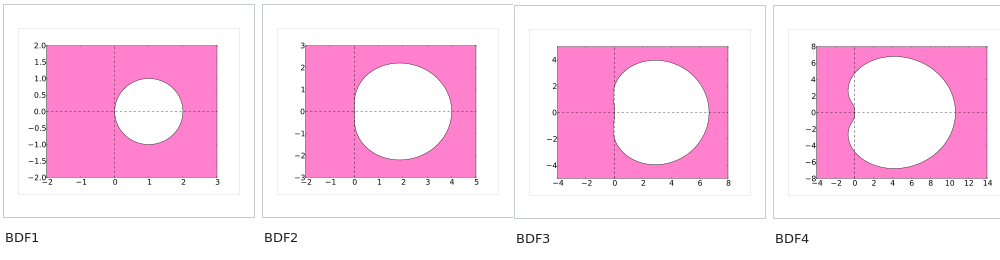
\includegraphics[width=\textwidth]{images/astab_bdf.png}
    \caption{\textit{An Introduction to Numerical Analysis}, Cambridge University Press}
\label{fig:astab_bdf}
\end{figure}

La partie rose de la figure \ref{fig:astab_bdf} indique les valeurs de A pour lesquelles la solution numérique de y tend vers 0 respectivement sous BDF1, BDF2, BDF3 et BDF4. On remarque donc que la méthode BDF est inconditionnellement A-Stable pour un ordre inférieur ou égal à 2 et conditionnellement stable sinon. Malgré cela, la méthode BDF reste plus stable que la méthode RK quelque soit son ordre.